% Options for packages loaded elsewhere
\PassOptionsToPackage{unicode}{hyperref}
\PassOptionsToPackage{hyphens}{url}
%
\documentclass[
]{book}
\usepackage{amsmath,amssymb}
\usepackage{iftex}
\ifPDFTeX
  \usepackage[T1]{fontenc}
  \usepackage[utf8]{inputenc}
  \usepackage{textcomp} % provide euro and other symbols
\else % if luatex or xetex
  \usepackage{unicode-math} % this also loads fontspec
  \defaultfontfeatures{Scale=MatchLowercase}
  \defaultfontfeatures[\rmfamily]{Ligatures=TeX,Scale=1}
\fi
\usepackage{lmodern}
\ifPDFTeX\else
  % xetex/luatex font selection
\fi
% Use upquote if available, for straight quotes in verbatim environments
\IfFileExists{upquote.sty}{\usepackage{upquote}}{}
\IfFileExists{microtype.sty}{% use microtype if available
  \usepackage[]{microtype}
  \UseMicrotypeSet[protrusion]{basicmath} % disable protrusion for tt fonts
}{}
\makeatletter
\@ifundefined{KOMAClassName}{% if non-KOMA class
  \IfFileExists{parskip.sty}{%
    \usepackage{parskip}
  }{% else
    \setlength{\parindent}{0pt}
    \setlength{\parskip}{6pt plus 2pt minus 1pt}}
}{% if KOMA class
  \KOMAoptions{parskip=half}}
\makeatother
\usepackage{xcolor}
\usepackage{color}
\usepackage{fancyvrb}
\newcommand{\VerbBar}{|}
\newcommand{\VERB}{\Verb[commandchars=\\\{\}]}
\DefineVerbatimEnvironment{Highlighting}{Verbatim}{commandchars=\\\{\}}
% Add ',fontsize=\small' for more characters per line
\usepackage{framed}
\definecolor{shadecolor}{RGB}{248,248,248}
\newenvironment{Shaded}{\begin{snugshade}}{\end{snugshade}}
\newcommand{\AlertTok}[1]{\textcolor[rgb]{0.94,0.16,0.16}{#1}}
\newcommand{\AnnotationTok}[1]{\textcolor[rgb]{0.56,0.35,0.01}{\textbf{\textit{#1}}}}
\newcommand{\AttributeTok}[1]{\textcolor[rgb]{0.13,0.29,0.53}{#1}}
\newcommand{\BaseNTok}[1]{\textcolor[rgb]{0.00,0.00,0.81}{#1}}
\newcommand{\BuiltInTok}[1]{#1}
\newcommand{\CharTok}[1]{\textcolor[rgb]{0.31,0.60,0.02}{#1}}
\newcommand{\CommentTok}[1]{\textcolor[rgb]{0.56,0.35,0.01}{\textit{#1}}}
\newcommand{\CommentVarTok}[1]{\textcolor[rgb]{0.56,0.35,0.01}{\textbf{\textit{#1}}}}
\newcommand{\ConstantTok}[1]{\textcolor[rgb]{0.56,0.35,0.01}{#1}}
\newcommand{\ControlFlowTok}[1]{\textcolor[rgb]{0.13,0.29,0.53}{\textbf{#1}}}
\newcommand{\DataTypeTok}[1]{\textcolor[rgb]{0.13,0.29,0.53}{#1}}
\newcommand{\DecValTok}[1]{\textcolor[rgb]{0.00,0.00,0.81}{#1}}
\newcommand{\DocumentationTok}[1]{\textcolor[rgb]{0.56,0.35,0.01}{\textbf{\textit{#1}}}}
\newcommand{\ErrorTok}[1]{\textcolor[rgb]{0.64,0.00,0.00}{\textbf{#1}}}
\newcommand{\ExtensionTok}[1]{#1}
\newcommand{\FloatTok}[1]{\textcolor[rgb]{0.00,0.00,0.81}{#1}}
\newcommand{\FunctionTok}[1]{\textcolor[rgb]{0.13,0.29,0.53}{\textbf{#1}}}
\newcommand{\ImportTok}[1]{#1}
\newcommand{\InformationTok}[1]{\textcolor[rgb]{0.56,0.35,0.01}{\textbf{\textit{#1}}}}
\newcommand{\KeywordTok}[1]{\textcolor[rgb]{0.13,0.29,0.53}{\textbf{#1}}}
\newcommand{\NormalTok}[1]{#1}
\newcommand{\OperatorTok}[1]{\textcolor[rgb]{0.81,0.36,0.00}{\textbf{#1}}}
\newcommand{\OtherTok}[1]{\textcolor[rgb]{0.56,0.35,0.01}{#1}}
\newcommand{\PreprocessorTok}[1]{\textcolor[rgb]{0.56,0.35,0.01}{\textit{#1}}}
\newcommand{\RegionMarkerTok}[1]{#1}
\newcommand{\SpecialCharTok}[1]{\textcolor[rgb]{0.81,0.36,0.00}{\textbf{#1}}}
\newcommand{\SpecialStringTok}[1]{\textcolor[rgb]{0.31,0.60,0.02}{#1}}
\newcommand{\StringTok}[1]{\textcolor[rgb]{0.31,0.60,0.02}{#1}}
\newcommand{\VariableTok}[1]{\textcolor[rgb]{0.00,0.00,0.00}{#1}}
\newcommand{\VerbatimStringTok}[1]{\textcolor[rgb]{0.31,0.60,0.02}{#1}}
\newcommand{\WarningTok}[1]{\textcolor[rgb]{0.56,0.35,0.01}{\textbf{\textit{#1}}}}
\usepackage{longtable,booktabs,array}
\usepackage{calc} % for calculating minipage widths
% Correct order of tables after \paragraph or \subparagraph
\usepackage{etoolbox}
\makeatletter
\patchcmd\longtable{\par}{\if@noskipsec\mbox{}\fi\par}{}{}
\makeatother
% Allow footnotes in longtable head/foot
\IfFileExists{footnotehyper.sty}{\usepackage{footnotehyper}}{\usepackage{footnote}}
\makesavenoteenv{longtable}
\usepackage{graphicx}
\makeatletter
\def\maxwidth{\ifdim\Gin@nat@width>\linewidth\linewidth\else\Gin@nat@width\fi}
\def\maxheight{\ifdim\Gin@nat@height>\textheight\textheight\else\Gin@nat@height\fi}
\makeatother
% Scale images if necessary, so that they will not overflow the page
% margins by default, and it is still possible to overwrite the defaults
% using explicit options in \includegraphics[width, height, ...]{}
\setkeys{Gin}{width=\maxwidth,height=\maxheight,keepaspectratio}
% Set default figure placement to htbp
\makeatletter
\def\fps@figure{htbp}
\makeatother
\setlength{\emergencystretch}{3em} % prevent overfull lines
\providecommand{\tightlist}{%
  \setlength{\itemsep}{0pt}\setlength{\parskip}{0pt}}
\setcounter{secnumdepth}{5}
\usepackage{booktabs}
\usepackage{amsthm}
\makeatletter
\def\thm@space@setup{%
  \thm@preskip=8pt plus 2pt minus 4pt
  \thm@postskip=\thm@preskip
}
\makeatother
\ifLuaTeX
  \usepackage{selnolig}  % disable illegal ligatures
\fi
\usepackage[]{natbib}
\bibliographystyle{apalike}
\IfFileExists{bookmark.sty}{\usepackage{bookmark}}{\usepackage{hyperref}}
\IfFileExists{xurl.sty}{\usepackage{xurl}}{} % add URL line breaks if available
\urlstyle{same}
\hypersetup{
  pdftitle={Temas Selectos de Análisis Numérico y Computación Científica: Computo científico para el análisis de datos},
  pdfauthor={Haydeé Peruyero},
  hidelinks,
  pdfcreator={LaTeX via pandoc}}

\title{Temas Selectos de Análisis Numérico y Computación Científica: Computo científico para el análisis de datos}
\author{Haydeé Peruyero}
\date{2024-02-06}

\begin{document}
\maketitle

{
\setcounter{tocdepth}{1}
\tableofcontents
}
\hypertarget{temas-selectos-de-anuxe1lisis-numuxe9rico-y-computaciuxf3n-cientuxedfica-computo-cientuxedfico-para-el-anuxe1lisis-de-datos}{%
\chapter{Temas Selectos de Análisis Numérico y Computación Científica: Computo científico para el análisis de datos}\label{temas-selectos-de-anuxe1lisis-numuxe9rico-y-computaciuxf3n-cientuxedfica-computo-cientuxedfico-para-el-anuxe1lisis-de-datos}}

Curso del posgrado conjunto en Ciencias Matemáticas PCCM UNAM UMICH 2024-2

\hypertarget{temario}{%
\section{Temario}\label{temario}}

\begin{enumerate}
\def\labelenumi{\arabic{enumi}.}
\item
  Git y Github
\item
  Shell
\item
  Python
\item
  SQL
\item
  Power BI
\item
  R
\item
  Estadística multivariada
\item
  Análisis de regresión
\end{enumerate}

\hypertarget{referencias}{%
\section{Referencias}\label{referencias}}

{[}1{]} Arnold, Jeremey. Learning Microsoft Power BI, O'Reilly Media, Inc.

{[}2{]} Beaulieu, Alan. Learning SQL, O'Reilly Media, Inc., 2020

{[}3{]} Bruce, Peter, Bruce, Andrew and Gedeck, Peter. Practical Statistics for Data Scientists, O'Reilly Media, Inc., 2020.

{[}4{]} Crawley, Michael J. The R book. John Wiley \& Sons, 2012.

{[}5{]} McKinney, Wes. Python for data analysis. O'Reilly Media, Inc., 2022.

{[}6{]} Nelli, Fabio. Python Data Analytics, Apress.

{[}7{]} Wade, Ryan. Advanced Analytics in Power BI with R and Python, Apress.

{[}8{]} Wickham, Hadley, and Garrett Grolemund. R for data science: import, tidy, transform, visualize, and
model data. O Reilly Media, Inc., 2016.

{[}9{]} Zamora Saiz, Alfonso, et al.~An Introduction to Data Analysis in R: Hands-on Coding, Data Mining,
Visualization and Statistics from Scratch., Springer (2020).

{[}10{]} Software Carpentry, The Unix Shell, \url{https://swcarpentry.github.io/shell-novice/}

\hypertarget{material-interesante}{%
\section{Material interesante}\label{material-interesante}}

\begin{itemize}
\tightlist
\item
  \href{https://bookdown.org/}{Bookdown}.
\item
  \href{https://swcarpentry.github.io/r-novice-gapminder/}{Software Carpentry}.
\item
  \href{https://swcarpentry.github.io/git-novice/14-supplemental-rstudio/}{Git}
\item
  \href{https://info5940.infosci.cornell.edu/setup/git/what-is-git/}{Why Git}
\item
  \href{https://bookdown.org/yihui/rmarkdown-cookbook/}{R Markdown Cookbook}
\item
  \href{http://www.sthda.com/english/wiki/data-visualization}{STHDA}
\item
  \href{https://bookdown.org/ndphillips/YaRrr/}{YaRrr! The Pirate's Guide to R}
\item
  \href{https://link.springer.com/book/10.1007/978-3-319-53019-2}{Learn ggplot2 Using Shiny App}
\item
  \href{https://link.springer.com/book/10.1007/978-0-387-98141-3}{Ggplot2: Elegant Graphics for Data Analysis}

  \begin{itemize}
  \tightlist
  \item
    \href{https://ggplot2-book.org/index.html}{Versión online}
  \end{itemize}
\item
  \href{https://www.springer.com/series/6991/books}{Use R! Colección Springer}
\item
  \href{https://link.springer.com/book/10.1007/978-0-387-75969-2}{Lattice: Multivariate Data Visualization with R}
\item
  \href{http://www.cookbook-r.com/}{R Graphics cookbook}
\end{itemize}

\hypertarget{datacamp}{%
\section{DataCamp}\label{datacamp}}

\begin{figure}
\centering

\includegraphics{img/regular.png}
\caption{DataCamp}
\end{figure}

\hypertarget{shell}{%
\chapter{Shell}\label{shell}}

Descargar \href{https://gitforwindows.org/}{git bash} para Windows o seguir las instrucciones de \href{https://carpentries.github.io/workshop-template/install_instructions/\#shell}{Software carpentries} para otros sistemas operativos.
Basado en la lección de \href{https://swcarpentry.github.io/shell-novice/}{The carpentries}

\hypertarget{navegar-en-archivos-y-directorios}{%
\section{Navegar en archivos y directorios}\label{navegar-en-archivos-y-directorios}}

Cuando abrimos una terminal por primera vez, vamos a ver un \textbf{prompt} (usualmente es \texttt{\$}) que nos indica que esta esperando los comandos. Después de teclear los comandos, debemos siempre presionar Enter.

\begin{Shaded}
\begin{Highlighting}[]
\ExtensionTok{$} 
\end{Highlighting}
\end{Shaded}

Para listar lo que hay en un directorio usamos el comando \texttt{ls}.

\begin{Shaded}
\begin{Highlighting}[]
\ExtensionTok{$}\NormalTok{ ls}
\end{Highlighting}
\end{Shaded}

\begin{Shaded}
\begin{Highlighting}[]
\NormalTok{Documents  Downloads  Music  Pictures  Videos}
\end{Highlighting}
\end{Shaded}

Al comando \texttt{ls} le podemos agregar unos \texttt{adjetivos} para hacer más comprensible su lectura. Por ejemplo, la opción \texttt{-F} nos indica si es una carpeta, un archivo, un link, etc.

\begin{Shaded}
\begin{Highlighting}[]
\ExtensionTok{$}\NormalTok{ ls }\AttributeTok{{-}F}
\end{Highlighting}
\end{Shaded}

\begin{Shaded}
\begin{Highlighting}[]
\NormalTok{ej.txt  Git/  PBI/  Python/  R/  Shell/  SQL/}
\end{Highlighting}
\end{Shaded}

Con la opción \texttt{-\/-help} podemos acceder a la ayuda del comando.

\begin{Shaded}
\begin{Highlighting}[]
\ExtensionTok{$}\NormalTok{ ls }\AttributeTok{{-}{-}help}
\end{Highlighting}
\end{Shaded}

Otras opciones que nos ayudan a entender la información que tenemos en el archivo son \texttt{-lh}, nos muestra los permisos del archivo o carpeta, tamaño, propietario, fecha, nombre. La opción \texttt{ls\ -a} nos muestra los archivos ocultos.

\textbf{Ejercicio:} ¿Qué hace la opción \texttt{-l}? ¿Cómo podemos listar en orden de creación e inverso?

Con el comando \texttt{ls} también podemos listar los archivos de cualquier otro directorio, solo debemos indicarle el directorio después del comando:

\begin{Shaded}
\begin{Highlighting}[]
\ExtensionTok{$}\NormalTok{ ls }\AttributeTok{{-}}\NormalTok{ F Shell }
\end{Highlighting}
\end{Shaded}

El comando \texttt{ls} solo nos esta listando lo que hay en los directorios. Si nos queremos mover a otro directorio, lo podemos hacer con el comando \texttt{cd} y especificando el directorio.

\begin{Shaded}
\begin{Highlighting}[]
\ExtensionTok{$}\NormalTok{ cd Shell}
\ExtensionTok{$}\NormalTok{ ls}
\end{Highlighting}
\end{Shaded}

\begin{Shaded}
\begin{Highlighting}[]
\NormalTok{data/  ej1.txt  ejercicios/}
\end{Highlighting}
\end{Shaded}

El comando \texttt{pwd} nos da la ruta en la que estamos.

\begin{Shaded}
\begin{Highlighting}[]
\ExtensionTok{$}\NormalTok{ pwd}
\end{Highlighting}
\end{Shaded}

\begin{Shaded}
\begin{Highlighting}[]
\NormalTok{/d/Users/hayde/Documents/Curso\_Comp\_Cien/Shell}
\end{Highlighting}
\end{Shaded}

Para movernos a un directorio arriba, colocamos después de \texttt{cd} dos puntos.

\begin{Shaded}
\begin{Highlighting}[]
\ExtensionTok{$}\NormalTok{ cd ..}
\end{Highlighting}
\end{Shaded}

Si no colocamos los dos puntos, el comando \texttt{cd} nos lleva al \texttt{/home/}.

\begin{Shaded}
\begin{Highlighting}[]
\ExtensionTok{$}\NormalTok{ cd }
\end{Highlighting}
\end{Shaded}

Otra forma de movernos de un directorio a otro es especificando la \emph{ruta absoluta}, es decir la ruta completa de a donde queremos movernos.

\begin{Shaded}
\begin{Highlighting}[]
\ExtensionTok{$}\NormalTok{ cd /d/Users/hayde/Documents/Curso\_comp\_Cien}
\end{Highlighting}
\end{Shaded}

\textbf{Ejercicio:} ¿Qué es una ruta relativa?

Otro opción útil que podemos usar con el comando \texttt{cd} es \texttt{-}.

\textbf{Ejercicio:} ¿A donde nos lleva \texttt{cd\ -}? y si volvemos a colocar \texttt{cd\ -} ¿a donde nos lleva? ¿Cuál es la diferencia entre \texttt{cd\ ..} y \texttt{cd\ -}?

La tilde \texttt{\textasciitilde{}}, shell la interpreta como el home del usuario, entonces si colocamos \texttt{cd\ \textasciitilde{}/directorio} sería lo mismo que \texttt{/home/directorio}. Por ejemplo:

\begin{Shaded}
\begin{Highlighting}[]
\ExtensionTok{$}\NormalTok{ cd \textasciitilde{}/Desktop}
\end{Highlighting}
\end{Shaded}

es lo mismo que

\begin{Shaded}
\begin{Highlighting}[]
\ExtensionTok{$}\NormalTok{ cd /c/Users/hayde/Desktop}
\end{Highlighting}
\end{Shaded}

\textbf{Ejercicio:} Supongamos que tenemos el siguiente árbol de datos en nuestra computadora y que estamos en \texttt{/Users/thing/}. ¿Si colocamos en la terminal \texttt{ls\ -F\ ../backup} que nos mostrará?

\begin{figure}
\centering
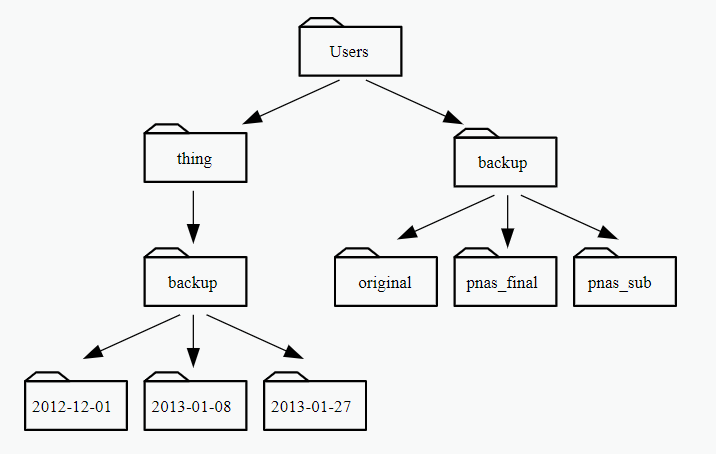
\includegraphics{img/ej_shell.png}
\caption{Ejercicio \href{https://swcarpentry.github.io/shell-novice/02-filedir.html}{SC}}
\end{figure}

\textbf{Ejercicio:} Explora las opciones \texttt{-s} y \texttt{-S}. ¿Hay diferencia entre mayúsculas y minúsculas?

La tecla Tab nos ayuda a completar los comando/rutas. Si la presionamos dos veces nos mostrará todas las posibles opciones.

\hypertarget{manipulaciuxf3n-de-archivos-y-directorios}{%
\section{Manipulación de archivos y directorios}\label{manipulaciuxf3n-de-archivos-y-directorios}}

Para crear directorios/carpetas desde la línea de comandos usamos el comando \texttt{mkdir\ nombre}. Vamos a crear la carpeta del curso. Es recomendable \textbf{no usar espacios en nombres de carpetas ni archivos}.

\begin{Shaded}
\begin{Highlighting}[]
\ExtensionTok{$}\NormalTok{ mkdir Curso\_Comp\_Cien}
\end{Highlighting}
\end{Shaded}

El comando \texttt{mkdir} nos permite crear más de un directorio y directorios anidados usando la opción \texttt{-p}.

\begin{Shaded}
\begin{Highlighting}[]
\ExtensionTok{$}\NormalTok{ mkdir }\AttributeTok{{-}p}\NormalTok{ Curso\_Comp\_Cien/Shell/data Curso\_Comp\_Cien/Shell/ejercicios}
\end{Highlighting}
\end{Shaded}

Para listar toda la estructura de nuestras carpetas podemos usar la opción \texttt{-FR} en el comando \texttt{ls}.

\begin{Shaded}
\begin{Highlighting}[]
\ExtensionTok{$}\NormalTok{ ls }\AttributeTok{{-}FR}
\end{Highlighting}
\end{Shaded}

Otra opción útil para listar toda la estructura de nuestro directorio es la opción \texttt{tree}, no viene instalado por default en los sistemas operativos. En Windows, si se instalo git/bash se puede usar con \texttt{tree.com}.

\begin{Shaded}
\begin{Highlighting}[]
\ExtensionTok{$}\NormalTok{ tree.com}
\end{Highlighting}
\end{Shaded}

\textbf{Nota:} Para descargar \texttt{tree} y que podamos ver la estructura de árbol con archivos y carpetas hacer lo siguiente:

\begin{enumerate}
\def\labelenumi{\arabic{enumi})}
\item
  Ir a la \href{https://gnuwin32.sourceforge.net/packages/tree.htm}{página} y descargar la versión que dice \emph{binaries}.
\item
  Extraer lo que hay en la carpeta \textbf{bin}.
\item
  Copiar el archivo \textbf{tree.exe} a la carpeta \texttt{/c/Program\_files/Git/usr/bin/}.
\item
  Para probarlo, solo colocar en la terminal \texttt{tree\ ruta}.
\end{enumerate}

Para crear un archivo usando el editor nano (si fue el que configuraron), se usa el comando \texttt{nano\ nombre.extension}.
Vamos a crear un archivo de prueba en la carpeta ejercicios y escribamos algo en el archivo.

\begin{Shaded}
\begin{Highlighting}[]
\ExtensionTok{$}\NormalTok{ cd Curso\_Comp\_Cien/}
\ExtensionTok{$}\NormalTok{ nano prueba.txt}
\end{Highlighting}
\end{Shaded}

Para guardar y salir del editor, usamos los comandos Ctrl+O o Ctrl+X seguido de \texttt{Yes} y enter.

Si en el archivo no guardaron nada, entonces no se creara. Una forma de crear archivos sin abrirlos es con el comando \texttt{touch}.

\begin{Shaded}
\begin{Highlighting}[]
\ExtensionTok{$}\NormalTok{ cd Shell/ejercicios}
\ExtensionTok{$}\NormalTok{ touch ../ej1.txt ej2.txt ../data/ej3.csv ../data/ej4.csv}
\end{Highlighting}
\end{Shaded}

Si checamos con \texttt{ls\ -l} los archivos o rutas que creamos, veremos que no tienen ningún tamaño.

Para mover archivos o renombrarlos, usamos el comando \texttt{mv} seguido del archivo que queremos mover/renombrar y la ruta a donde lo moveremos o el nuevo nombre del archivo.

\begin{Shaded}
\begin{Highlighting}[]
\ExtensionTok{$}\NormalTok{ pwd}
\ExtensionTok{$}\NormalTok{ mv ej2.txt ejercicio2.txt}
\end{Highlighting}
\end{Shaded}

Lo anterior esta cambiándole el nombre al archivo \texttt{ej2.txt} por \texttt{ejercicio2.txt}.

Si estamos en un directorio y queremos mover un archivo de otro directorio al directorio actual, podemos hacerlo especificando como primer argumento la ruta y nombre del archivo a mover y como segundo argumento un punto \texttt{.}.

\begin{Shaded}
\begin{Highlighting}[]
\ExtensionTok{$}\NormalTok{ mv ../ej1.txt .}
\end{Highlighting}
\end{Shaded}

O especificando la ruta completa.

\begin{Shaded}
\begin{Highlighting}[]
\ExtensionTok{$}\NormalTok{ cd ..}
\ExtensionTok{$}\NormalTok{ mv data/ej3.csv ejercicios/.}
\end{Highlighting}
\end{Shaded}

Para copiar archivos, usamos el comando \texttt{cp} seguido por la ruta del archivo a copiar y la ruta del archivo a donde se copiará. Movámonos a la carpeta \texttt{Shell/ejercicios}.

\begin{Shaded}
\begin{Highlighting}[]
\ExtensionTok{$}\NormalTok{ pwd}
\ExtensionTok{$}\NormalTok{ cp ejercicio2.txt ../ej2.txt}
\ExtensionTok{$}\NormalTok{ ls }\AttributeTok{{-}FR}
\end{Highlighting}
\end{Shaded}

Si usamos la opción \texttt{-r} (\emph{recursivo}) en el comando \texttt{cp} podemos copiar un directorio completo y todos sus elementos.

\begin{Shaded}
\begin{Highlighting}[]
\ExtensionTok{$}\NormalTok{ cd ejercicios}
\ExtensionTok{$}\NormalTok{ cp }\AttributeTok{{-}r}\NormalTok{ ../data .}
\end{Highlighting}
\end{Shaded}

\textbf{Ejercicio:} ¿Cual es el output de la siguiente colección de comandos?

\begin{Shaded}
\begin{Highlighting}[]
\ExtensionTok{$}\NormalTok{ pwd}
\end{Highlighting}
\end{Shaded}

\begin{Shaded}
\begin{Highlighting}[]
\NormalTok{/Users/haydee/Curso}
\end{Highlighting}
\end{Shaded}

\begin{Shaded}
\begin{Highlighting}[]
\ExtensionTok{$}\NormalTok{ ls }\AttributeTok{{-}F}
\end{Highlighting}
\end{Shaded}

\begin{Shaded}
\begin{Highlighting}[]
\NormalTok{archivo.txt carpeta/}
\end{Highlighting}
\end{Shaded}

\begin{Shaded}
\begin{Highlighting}[]
\ExtensionTok{$}\NormalTok{ mkdir carpeta2}
\ExtensionTok{$}\NormalTok{ mv archivo.txt carpeta2/}
\ExtensionTok{$}\NormalTok{ cd carpeta2}
\ExtensionTok{$}\NormalTok{ cp archivo.txt ../carpeta/archivo\_respaldo.txt}
\ExtensionTok{$}\NormalTok{ cd ..}
\ExtensionTok{$}\NormalTok{ ls }\AttributeTok{{-}FR}
\end{Highlighting}
\end{Shaded}

Para borrar archivos usamos el comando \texttt{rm}, hay que tener cuidado cuando lo usemos ya que \textbf{borra definitivamente} los archivos o carpetas.

\begin{Shaded}
\begin{Highlighting}[]
\ExtensionTok{$}\NormalTok{ cd Shell}
\ExtensionTok{$}\NormalTok{ rm ejercicios/ejercicio2.txt}
\ExtensionTok{$}\NormalTok{ ls ejercicios/}
\end{Highlighting}
\end{Shaded}

Una forma segura de borrar archivos es usando la opción \texttt{-i}, con esto nos saldrá un mensaje preguntando si en verdad deseamos borrar el archivo. Para confirmar debemos colocar \texttt{y}.

\begin{Shaded}
\begin{Highlighting}[]
\ExtensionTok{$}\NormalTok{ rm }\AttributeTok{{-}i}\NormalTok{ /data/ej3.csv}
\end{Highlighting}
\end{Shaded}

\begin{Shaded}
\begin{Highlighting}[]
\NormalTok{rm: remove regular empty file \textquotesingle{}ej3.txt\textquotesingle{}?}
\end{Highlighting}
\end{Shaded}

Si queremos borrar una carpeta, debemos hacerlo con la opción \texttt{-r}, de lo contrario obtendremos un error.

\begin{Shaded}
\begin{Highlighting}[]
\ExtensionTok{$}\NormalTok{ rm data}
\end{Highlighting}
\end{Shaded}

\begin{Shaded}
\begin{Highlighting}[]
\ExtensionTok{$}\NormalTok{ rm }\AttributeTok{{-}r}\NormalTok{ data}
\end{Highlighting}
\end{Shaded}

Para mover/copiar/eliminar multiples archivos a la vez, podemos enumerarlos todos o usar comodines/patrones que sigan estos elementos. Supongamos que tenemos una lista de archivos todos con terminación \texttt{.txt}, entonces para borrarlos podemos usar \texttt{rm\ *.txt}. El \texttt{*} nos indica todo lo que este antes de \texttt{.txt}.

\begin{Shaded}
\begin{Highlighting}[]
\ExtensionTok{$}\NormalTok{ cd Shell/}
\ExtensionTok{$}\NormalTok{ touch prueba1.txt prueba2.txt prueba3.txt prueba4.txt prueba5.txt}
\ExtensionTok{$}\NormalTok{ rm }\PreprocessorTok{*}\NormalTok{.txt}
\end{Highlighting}
\end{Shaded}

Otro comodín que podemos usar es \texttt{?}, pero este denota solo 1 espacio. Por ejemplo:

\begin{Shaded}
\begin{Highlighting}[]
\ExtensionTok{$}\NormalTok{ cd Shell/}
\ExtensionTok{$}\NormalTok{ touch prueba1.txt prueba2.txt prueba3.txt prueba4.txt prueba5.txt}
\ExtensionTok{$}\NormalTok{ rm prueba}\PreprocessorTok{?}\NormalTok{.txt}
\end{Highlighting}
\end{Shaded}

\begin{Shaded}
\begin{Highlighting}[]
\ExtensionTok{$}\NormalTok{ cd Shell/}
\ExtensionTok{$}\NormalTok{ touch prueba1.txt prueba2.txt prueba3.txt prueba4.txt prueba5.txt}
\ExtensionTok{$}\NormalTok{ rm prue}\PreprocessorTok{???}\NormalTok{.txt}
\end{Highlighting}
\end{Shaded}

\textbf{Ejercicio:} Supon que en el directorio \texttt{data} tienes dos archivos. ¿Cuál de los siguientes comandos te daría como resultado: \texttt{ethane.pdb} \texttt{methane.pdb}.

\begin{enumerate}
\def\labelenumi{\arabic{enumi})}
\item
  \texttt{ls\ *t*ane.pdb}
\item
  \texttt{ls\ *t?ne.*}
\item
  \texttt{ls\ *t??ne.pdb}
\item
  ls ethane.*
\end{enumerate}

\hypertarget{tuberuxedas-y-filtros}{%
\section{Tuberías y filtros}\label{tuberuxedas-y-filtros}}

Vamos a usar los archivos de prueba de la lección de Shell de Software Carpentry. Descargarlos en el directorio que creamos que se llama \href{https://swcarpentry.github.io/shell-novice/data/shell-lesson-data.zip}{Shell}.

Vamos a explorar los archivos que están en la carpeta \texttt{excercise-data/alkanes}. Para contar cuantos palabras, líneas o caracteres tiene un archivo, usamos el comando \texttt{wc} que viene de \texttt{word\ count}.

\begin{Shaded}
\begin{Highlighting}[]
\ExtensionTok{$}\NormalTok{ ls}
\end{Highlighting}
\end{Shaded}

\begin{Shaded}
\begin{Highlighting}[]
\NormalTok{cubane.pdb  ethane.pdb  methane.pdb  octane.pdb  pentane.pdb  propane.pdb}
\end{Highlighting}
\end{Shaded}

\begin{Shaded}
\begin{Highlighting}[]
\ExtensionTok{$}\NormalTok{ wc cubane.pdb}
\end{Highlighting}
\end{Shaded}

\begin{Shaded}
\begin{Highlighting}[]
\NormalTok{20  156 1158 cubane.pdb}
\end{Highlighting}
\end{Shaded}

El primer número es el número de líneas del archivo, el segundo la cantidad de palabras y el tercero la cantidad de caracteres.

Si usamos alguna de los comodines, por ejemplo \texttt{*.pdb} con el comando \texttt{wc}, nos va a regresar la información de todos los archivos.

\begin{Shaded}
\begin{Highlighting}[]
\ExtensionTok{$}\NormalTok{ wc }\PreprocessorTok{*}\NormalTok{.pdb}
\end{Highlighting}
\end{Shaded}

Notemos que en la última fila tenemos los totales de todos los archivos. Accedamos a la ayuda del comando con \texttt{help}.

\begin{Shaded}
\begin{Highlighting}[]
\ExtensionTok{$}\NormalTok{ wc }\AttributeTok{{-}{-}help}
\end{Highlighting}
\end{Shaded}

\textbf{Ejercicio:} ¿Cuál opción nos permite extraer solo la cantidad de líneas del archivo?

\begin{Shaded}
\begin{Highlighting}[]
\ExtensionTok{$}\NormalTok{ wc }\AttributeTok{{-}l} \PreprocessorTok{*}\NormalTok{.pdb}
\end{Highlighting}
\end{Shaded}

Si por error olvidamos colocar el nombre del archivo o cualquier otra cosa después del comando, la consola se quedará esperando una instrucción, para salir de esto basta presionar Ctrl+C.

Ya sabemos como extraer cierta información de nuestros archivos, pero supongamos que queremos guardarlo ahora en algún otro archivo para después analizarlo. El símbolo \texttt{\textgreater{}} redirige el resultado de los comandos usados a algún archivo.

\begin{Shaded}
\begin{Highlighting}[]
\ExtensionTok{$}\NormalTok{ wc }\AttributeTok{{-}l} \PreprocessorTok{*}\NormalTok{.pdb }\OperatorTok{\textgreater{}}\NormalTok{ lineas.txt}
\end{Highlighting}
\end{Shaded}

Para solo visualizar el contenido de un archivo sin entrar al editor de texto, podemos usar el comando \texttt{cat} seguido del nombre del archivo.

\begin{Shaded}
\begin{Highlighting}[]
\ExtensionTok{$}\NormalTok{ cat lineas.txt}
\end{Highlighting}
\end{Shaded}

Otro comando que puede resultar más útil para mostrar el contenido de un archivo es \texttt{less}, la diferencia con \texttt{cat} es que este último muestra todo el contenido en la pantalla, lo cual puede dificultar su lectura e inspección, mientras que \texttt{less} muestra una parte del contenido y de forma ordenada, si queremos seguir viendo el contenido podemos usar la tecla de espacio, b y para salir usamos la letra \texttt{q}.

Ya guardamos la información de la cantidad de líneas, pero supongamos que queremos saber cual archivo tiene la mayor cantidad de líneas o menor. Para hacer esto nos sirve el comando \texttt{sort}.

\begin{Shaded}
\begin{Highlighting}[]
\ExtensionTok{$}\NormalTok{ cd ..}
\ExtensionTok{$}\NormalTok{ sort numbers.txt}
\end{Highlighting}
\end{Shaded}

Si a \texttt{sort} le agregamos la opción \texttt{-n}, nos los ordena en numericamente en lugar de alfabeticamente.

\begin{Shaded}
\begin{Highlighting}[]
\ExtensionTok{$}\NormalTok{ sort }\AttributeTok{{-}n}\NormalTok{ numbers.txt}
\end{Highlighting}
\end{Shaded}

\textbf{Ejercicio:} De los archivos que están en la carpeta \texttt{alkane}, ¿cuál tiene la menor cantidad de líneas?

También podemos redirigir esta información a otro archivo y de ahí extraer la información.

\begin{Shaded}
\begin{Highlighting}[]
\ExtensionTok{$}\NormalTok{ sort }\AttributeTok{{-}n}\NormalTok{ lineas.txt }\OperatorTok{\textgreater{}}\NormalTok{ lineas\_ordenadas.txt}
\end{Highlighting}
\end{Shaded}

El comando \texttt{head} nos ayuda a extraer las primeras \texttt{n} líneas de nuestro archivo. Por ejemplo, para extraer la primera línea del archivo \texttt{lineas\_ordenadas.txt} y así saber cual archivo tenía la menor cantidad de líneas usaríamos \texttt{head\ -n\ 1}.

\begin{Shaded}
\begin{Highlighting}[]
\ExtensionTok{$}\NormalTok{ head }\AttributeTok{{-}n}\NormalTok{ 1 lineas\_ordenadas.txt}
\end{Highlighting}
\end{Shaded}

El comando \texttt{echo} nos ayuda a imprimir en la consola caracteres.

\begin{Shaded}
\begin{Highlighting}[]
\ExtensionTok{$}\NormalTok{ echo Hola}
\end{Highlighting}
\end{Shaded}

\textbf{Ejercicio:} Realiza las siguientes instrucciones dos veces cada una. Explora las diferencias. ¿Qué hace el operador \texttt{\textgreater{}\textgreater{}}?

\begin{Shaded}
\begin{Highlighting}[]
\ExtensionTok{$}\NormalTok{ echo hola }\OperatorTok{\textgreater{}}\NormalTok{ test1.txt}
\end{Highlighting}
\end{Shaded}

\begin{Shaded}
\begin{Highlighting}[]
\ExtensionTok{$}\NormalTok{ echo hola }\OperatorTok{\textgreater{}\textgreater{}}\NormalTok{ test2.txt}
\end{Highlighting}
\end{Shaded}

El comando \texttt{tail} es similar al comando \texttt{head}, nos muestra las últimas \texttt{n} filas del archivo.

\textbf{Ejercicio:} Considera el archivo \texttt{/exercise-data/animal-counts/animals.csv}. Después de aplicar los siguientes dos comandos, ¿qué hay en el archivo \texttt{animals-subset.csv}?

\begin{Shaded}
\begin{Highlighting}[]
\ExtensionTok{$}\NormalTok{ head }\AttributeTok{{-}n}\NormalTok{ 3 animals.csv }\OperatorTok{\textgreater{}}\NormalTok{ animals{-}subset.csv}
\ExtensionTok{$}\NormalTok{ tail }\AttributeTok{{-}n}\NormalTok{ 2 animals.csv }\OperatorTok{\textgreater{}\textgreater{}}\NormalTok{ animals{-}subset.csv}
\end{Highlighting}
\end{Shaded}

\hypertarget{tuberuxedas}{%
\subsection{Tuberías}\label{tuberuxedas}}

Además de redirigir los output de los comandos que hemos ocupado, también podríamos anidarlos y al final mandarlo a un archivo. Para hacer esto se usan \textbf{tuberías} y su símbolo es \texttt{\textbar{}}. Por ejemplo:

\begin{Shaded}
\begin{Highlighting}[]
\ExtensionTok{$}\NormalTok{ sort }\AttributeTok{{-}n}\NormalTok{ lineas.txt }\KeywordTok{|} \FunctionTok{head} \AttributeTok{{-}n}\NormalTok{ 1}
\end{Highlighting}
\end{Shaded}

En esta instrucción le estamos diciendo a la consola que primero nos ordene lo que hay en el archivo líneas en orden númerico y después que nos muestre la primera línea. De esta forma nos evitamos por ejemplo el haber creado el archivo \texttt{lineas\_ordenadas.txt}.

Podemos anidar varias instrucciones a la vez. Por ejemplo, podríamos pedirle a la consola la cantidad de líneas de los archivos \texttt{*.pdb}, pedirle que las ordene numericamente y después que extraiga la primera línea.

\begin{Shaded}
\begin{Highlighting}[]
\ExtensionTok{$}\NormalTok{ wc }\AttributeTok{{-}l} \PreprocessorTok{*}\NormalTok{.pdb }\KeywordTok{|} \FunctionTok{sort} \AttributeTok{{-}n} \KeywordTok{|} \FunctionTok{head} \AttributeTok{{-}n}\NormalTok{ 1}
\end{Highlighting}
\end{Shaded}

\textbf{Ejercicio:} De los archivos que están en la carpeta \texttt{alkanes}, obten los 3 archivos con la menor cantidad de líneas.

\textbf{Ejercicio:} Explora el archivo \texttt{exercise-data/animals-counts/animals.csv}. ¿Cuál será el resultado de la siguiente instrucción?

\begin{Shaded}
\begin{Highlighting}[]
\ExtensionTok{$}\NormalTok{ cat animals.csv }\KeywordTok{|} \FunctionTok{head} \AttributeTok{{-}n}\NormalTok{ 5 }\KeywordTok{|} \FunctionTok{tail} \AttributeTok{{-}n}\NormalTok{ 3 }\KeywordTok{|} \FunctionTok{sort} \AttributeTok{{-}r} \OperatorTok{\textgreater{}}\NormalTok{ final.txt}
\end{Highlighting}
\end{Shaded}

El comando \texttt{cut} nos ayuda a extrar/cortar ciertas columnas de nuestros archivos. Por ejemplo, \texttt{cut\ -d\ ,\ -f\ 2\ archivo} nos está indicando que del archivo queremos cortar por caracteres \texttt{,} (eso hace \texttt{-d\ ,}) y que queremos extraer la segunda columna (\texttt{-f\ 2}).

\begin{Shaded}
\begin{Highlighting}[]
\ExtensionTok{$}\NormalTok{ cut }\AttributeTok{{-}d}\NormalTok{ , }\AttributeTok{{-}f}\NormalTok{ 2 animals.csv}
\end{Highlighting}
\end{Shaded}

Si quisieramos extraer los animales únicos de ese archivo, podemos usar el comando \texttt{uniq}.

\begin{Shaded}
\begin{Highlighting}[]
\ExtensionTok{$}\NormalTok{ cut }\AttributeTok{{-}d}\NormalTok{ , }\AttributeTok{{-}f}\NormalTok{ 2 animals.csv }\KeywordTok{|} \FunctionTok{sort} \KeywordTok{|} \FunctionTok{uniq}
\end{Highlighting}
\end{Shaded}

\textbf{Ejercicio:} ¿Porqué se necesita colocar el \texttt{sort} antes del \texttt{uniq}?

\textbf{Ejercicio:} Si quisiéramos ver cuantos animales hay de cada tipo, ¿que instrucción tendríamos que usar?

\hypertarget{ciclos}{%
\section{Ciclos}\label{ciclos}}

Los ciclos nos ayudan a repetir comandos o un conjunto de comandos para cada elemento de una lista. La estructura del ciclo \texttt{for} es como sigue:

\begin{Shaded}
\begin{Highlighting}[]
\ControlFlowTok{for}\NormalTok{ elemento }\KeywordTok{in}\NormalTok{ lista}
\ControlFlowTok{do} 
  \ExtensionTok{operacion/comando} \VariableTok{$elemento}
\ControlFlowTok{done}
\end{Highlighting}
\end{Shaded}

La palabra \texttt{for} indica el comienzo del ciclo, la palabra \texttt{do} nos indica que es lo que se va a ejecutar y su comienzo y la palabra \texttt{done} indica el fin del ciclo.

Exploremos lo que hay en la carpeta \texttt{\textasciitilde{}/Shell/shell-lesson-data/exercise-data/creatures}. Listemos las primeras 5 filas de cada archivo.

\begin{Shaded}
\begin{Highlighting}[]
\ExtensionTok{$}\NormalTok{ head }\AttributeTok{{-}n}\NormalTok{ 5 basilisk.dat minotaur.dat unicorn.dat}
\end{Highlighting}
\end{Shaded}

Supongamos que queremos ver la clasificación de cada especie que se encuentra en la segunda línea de cada archivo. Una forma de hacerlo es con \texttt{head\ -n\ 2}, pero de esta forma también estamos viendo su nombre común, entonces vamos a hacerlo con un ciclo. Lo primero que tendríamos que hacer es usar justo \texttt{head\ -n\ 2} y al resultado de esto, si le pedimos la última línea ya solo veríamos la clasificación, entonces usamos un \texttt{tail\ -n\ 1}.

\begin{Shaded}
\begin{Highlighting}[]
\ExtensionTok{$}\NormalTok{ for filename in }\PreprocessorTok{*}\NormalTok{.dat}
\OperatorTok{\textgreater{}}\NormalTok{ do}
\OperatorTok{\textgreater{}}\NormalTok{   echo }\VariableTok{$filename}
\OperatorTok{\textgreater{}}\NormalTok{   head }\ExtensionTok{{-}n}\NormalTok{ 2 }\VariableTok{$filename} \KeywordTok{|} \FunctionTok{tail} \AttributeTok{{-}n}\NormalTok{ 1}
\OperatorTok{\textgreater{}}\NormalTok{ done}
\end{Highlighting}
\end{Shaded}

Notemos que cuando empezamos a teclear nuestro ciclo, el prompt cambia de \texttt{\$} a \texttt{\textgreater{}}, esto indica que está esperando que continuemos el ciclo. También podemos usar \texttt{;} para continuar las instrucciones en una misma fila.

Dentro de los ciclos, las variables las mandamos a llamar con \texttt{\$}, en el ejemplo, cuando ocupamos \texttt{\$filename} estamos mandando a llamar la variable \texttt{filename} que definimos al inicio del ciclo. Es muy usual también encerrar entre llaves los nombres de las variables para delimitar el nombre, en el ejemplo, \texttt{\$filename} sería equivalente a \texttt{\$\{filename\}}.

\textbf{Ejercicio:} Crea un ciclo que muestre en pantalla (echo) todos los números del 0 al 9.

\textbf{Ejercicio:} Ve a la carpeta \texttt{shell-lesson-data/exercise-data/alkanes} y lista lo que hay.
1) ¿Cuál es el output del siguiente código?

\begin{Shaded}
\begin{Highlighting}[]
\ExtensionTok{$}\NormalTok{ for datafile in }\PreprocessorTok{*}\NormalTok{.pdb}
\OperatorTok{\textgreater{}}\NormalTok{ do}
\OperatorTok{\textgreater{}}\NormalTok{     ls }\ExtensionTok{*.pdb}
\OperatorTok{\textgreater{}}\NormalTok{ done}
\end{Highlighting}
\end{Shaded}

\begin{enumerate}
\def\labelenumi{\arabic{enumi})}
\setcounter{enumi}{1}
\tightlist
\item
  ¿Y de este código?
\end{enumerate}

\begin{Shaded}
\begin{Highlighting}[]
\ExtensionTok{$}\NormalTok{ for datafile in }\PreprocessorTok{*}\NormalTok{.odb}
\OperatorTok{\textgreater{}}\NormalTok{ do }
\OperatorTok{\textgreater{}}\NormalTok{     ls }\VariableTok{$datafile}
\OperatorTok{\textgreater{}}\NormalTok{ done}
\end{Highlighting}
\end{Shaded}

Explica las diferencias.

\textbf{Ejercicio:} En el directorio \texttt{shell-lesson-data/exercise-data/alkanes}, ¿cuál sería el output del siguiente código?

\begin{Shaded}
\begin{Highlighting}[]
\ExtensionTok{$}\NormalTok{ for filename in c}\PreprocessorTok{*}
\OperatorTok{\textgreater{}}\NormalTok{ do}
\OperatorTok{\textgreater{}}\NormalTok{     ls }\VariableTok{$filename}
\OperatorTok{\textgreater{}}\NormalTok{ done}
\end{Highlighting}
\end{Shaded}

Y si en lugar de \texttt{c*} usamos \emph{c}?

Dentro de un ciclo también podemos pedir guardar archivos.

\textbf{Ejercicio:} Explora el siguiente código. ¿Cuál es el efecto de guardar en este ciclo?

\begin{Shaded}
\begin{Highlighting}[]
\ExtensionTok{$}\NormalTok{ for alkanes in }\PreprocessorTok{*}\NormalTok{.pdb}
\OperatorTok{\textgreater{}}\NormalTok{ do}
\OperatorTok{\textgreater{}}\NormalTok{     echo }\VariableTok{$alkanes}
\OperatorTok{\textgreater{}}\NormalTok{     cat }\VariableTok{$alkanes} \OperatorTok{\textgreater{}}\NormalTok{ alkanes.pdb}
\OperatorTok{\textgreater{}}\NormalTok{ done}
\end{Highlighting}
\end{Shaded}

¿Cuál sería la diferencia si usamos ahora \texttt{\textgreater{}\textgreater{}}?

\textbf{Ejercicio:} Crea un ciclo que muestre las últimas 20 líneas de cada archivo en la carpeta \texttt{creatures}.

Como ya mencionamos, no es recomendable usar espacios ni caracteres especiales en nombres de archivos o carpetas. Si fuera el caso de que nuestros archivos tienen espacios, entonces deberíamos pasarlos al ciclo for encerrados entre comillas los nombres. Por ejemplo, supongamos que tenemos los archivos \texttt{archivo\ 1.txt} y \texttt{archivo\ 2.txt}. Para leerlos en el ciclo for tendríamos que usar la siguiente sintaxis.

\begin{Shaded}
\begin{Highlighting}[]
\ExtensionTok{$}\NormalTok{ for filename in }\StringTok{"archivo 1.txt"} \StringTok{"archivo 2.txt"}
\OperatorTok{\textgreater{}}\NormalTok{ do}
\OperatorTok{\textgreater{}}\NormalTok{     head }\ExtensionTok{{-}n20} \StringTok{"}\VariableTok{$filename}\StringTok{"} \KeywordTok{|} \FunctionTok{tail} \AttributeTok{{-}n5} 
\OperatorTok{\textgreater{}}\NormalTok{ done}
\end{Highlighting}
\end{Shaded}

Supongamos que queremos modificar nuestros archivos que se encuentran en la carpeta \texttt{creatures} pero que antes queremos respaldarlos en otros archivos llamados \texttt{original-basilisk.dat}, \texttt{original-unicorn.dat} y \texttt{original-minotaur.dat}. Una forma de hacerlo sería copiarlos a nuevos archivos con esos nombres, pero si no lo queremos hacer manualmente, ¿qué pasa si usamos el siguiente código?

\begin{Shaded}
\begin{Highlighting}[]
\ExtensionTok{$}\NormalTok{ cp }\PreprocessorTok{*}\NormalTok{.dat original{-}}\PreprocessorTok{*}\NormalTok{.dat}
\end{Highlighting}
\end{Shaded}

Esto nos va a dar un error porque el comando \texttt{cp} estaría esperando que \texttt{original-} sea una carpeta y no lo es, no existe esa carpeta. Entonces lo que podemos hacer es usar un ciclo.

\textbf{Ejercicio:} Crea un ciclo \texttt{for} que copie los dos archivos a dos nuevos archivos llamados \texttt{original-basilisk.dat}, \texttt{original-unicorn.dat} y \texttt{original-minotaur.dat}.

El comando \texttt{cp} no nos muestra en pantalla ningún output. Si quisieramos ver que en efecto se esta realizando la copia de estos archivos podemos usar el comando \texttt{echo} y pedir que nos diga como ``se copio el archivo \$filename''. Usar \texttt{echo} de esta forma es una buena práctica de realizar lo que se llama \textbf{debugging}.

\begin{Shaded}
\begin{Highlighting}[]
\ExtensionTok{$}\NormalTok{ for filename in }\PreprocessorTok{*}\NormalTok{.dat}
\OperatorTok{\textgreater{}}\NormalTok{ do}
\OperatorTok{\textgreater{}}\NormalTok{     echo }\FunctionTok{cp} \VariableTok{$filename}\NormalTok{ original{-}}\VariableTok{$filename}
\OperatorTok{\textgreater{}}\NormalTok{ done}
\end{Highlighting}
\end{Shaded}

\begin{figure}
\centering
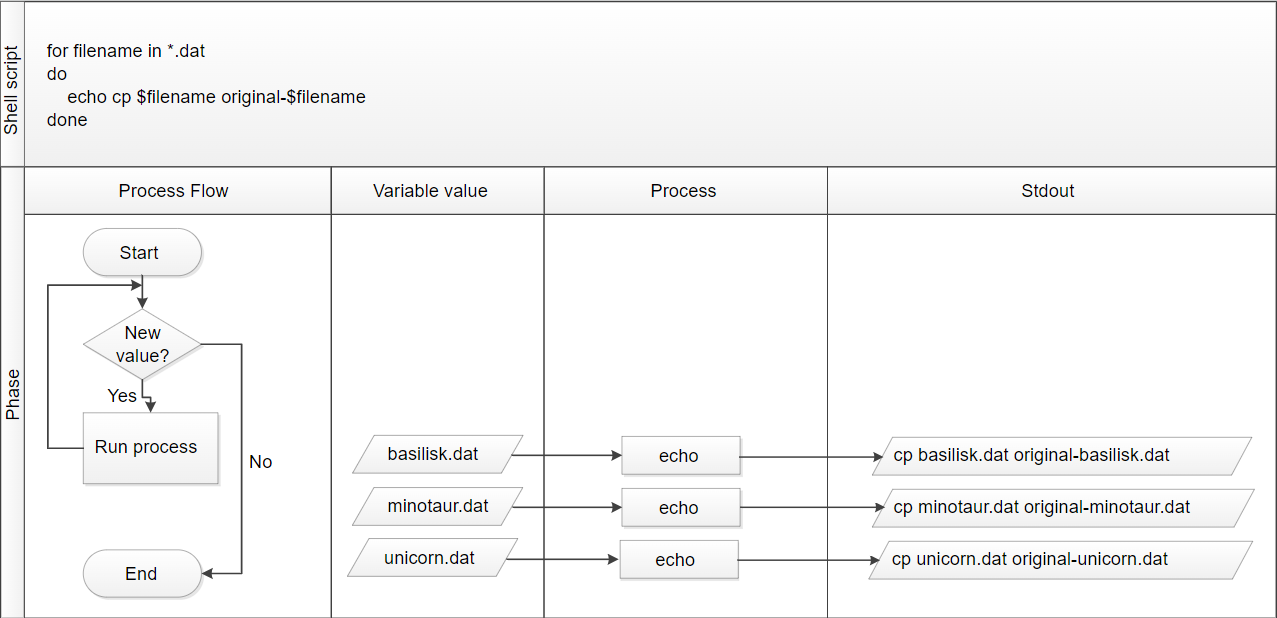
\includegraphics{D:/Users/hayde/Documents/R_sites/Computo_Cientifico/img/shell_script_for_loop_flow_chart.png}
\caption{Debugging}
\end{figure}

\textbf{Ejercicio:} Supongamos que queremos previsualizar los comandos que el siguiente ciclo va a realizar en lugar de correrlo primero para asegurarnos de que está haciendo lo que queremos.

\begin{Shaded}
\begin{Highlighting}[]
\ExtensionTok{$}\NormalTok{ for filename in }\PreprocessorTok{*}\NormalTok{.pdb}
\OperatorTok{\textgreater{}}\NormalTok{ do}
\OperatorTok{\textgreater{}}\NormalTok{     cat }\VariableTok{$filename} \OperatorTok{\textgreater{}\textgreater{}}\NormalTok{ all.pdb}
\OperatorTok{\textgreater{}}\NormalTok{ done}
\end{Highlighting}
\end{Shaded}

¿Cuál de los siguientes dos códigos sería el correcto para revisar los comando a ejecutarse con el ciclo?

\begin{Shaded}
\begin{Highlighting}[]
\CommentTok{\# Versión 1}
\ExtensionTok{$}\NormalTok{ for filename in }\PreprocessorTok{*}\NormalTok{.pdb}
\OperatorTok{\textgreater{}}\NormalTok{ do}
\OperatorTok{\textgreater{}}\NormalTok{     echo }\FunctionTok{cat} \VariableTok{$filename} \OperatorTok{\textgreater{}\textgreater{}}\NormalTok{ all.pdb}
\OperatorTok{\textgreater{}}\NormalTok{ done}
\end{Highlighting}
\end{Shaded}

\begin{Shaded}
\begin{Highlighting}[]
\CommentTok{\# Versión 2}
\ExtensionTok{$}\NormalTok{ for filename in }\PreprocessorTok{*}\NormalTok{.pdb}
\OperatorTok{\textgreater{}}\NormalTok{ do}
\OperatorTok{\textgreater{}}\NormalTok{    echo }\StringTok{"cat }\VariableTok{$filename}\StringTok{ \textgreater{}\textgreater{} all.pdb"}
\OperatorTok{\textgreater{}}\NormalTok{ done}
\end{Highlighting}
\end{Shaded}

Corre los dos códigos y explora el contenido del archivo \texttt{all.pdb}.

Supongamos que queremos crear una estructura de directorios como sigue, para cada compuesto y cada temperatura queremos una carpeta para ir guardando ahí sus resultados, y que cada carpeta se llame \texttt{compuesto-temperatura}, ¿cómo podemos hacer esto? Una opción son los ciclos anidados.

\begin{figure}
\centering
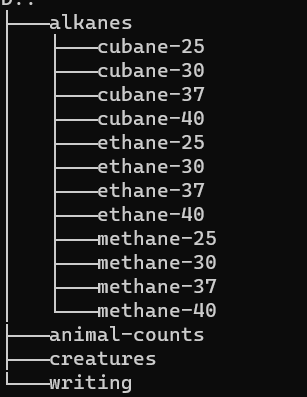
\includegraphics{D:/Users/hayde/Documents/R_sites/Computo_Cientifico/img/estructura-alkanes.png}
\caption{estructura-experimentos}
\end{figure}

\begin{Shaded}
\begin{Highlighting}[]
\ExtensionTok{$}\NormalTok{ for species in cubane ethane methane }
\OperatorTok{\textgreater{}}\NormalTok{ do}
\OperatorTok{\textgreater{}}\NormalTok{     for }\ExtensionTok{temperature}\NormalTok{ in 25 30 37 40}
\OperatorTok{\textgreater{}}\NormalTok{     do}
\OperatorTok{\textgreater{}}\NormalTok{         mkdir }\VariableTok{$species}\ExtensionTok{{-}}\VariableTok{$temperature}
\OperatorTok{\textgreater{}}\NormalTok{     done}
\OperatorTok{\textgreater{}}\NormalTok{ done}
\end{Highlighting}
\end{Shaded}

Algunos comandos útiles para ver el historial de comadnos.

\begin{itemize}
\item
  \texttt{history} nos muestra el historial de comandos.
\item
  Ctrl+R nos muestra la leyenda \texttt{reverse-i-search}, esto indica que está esperando que nosotros coloquemos una palabra y buscará por el último comando con esa palabra.
\item
  \texttt{history} + \texttt{!123} nos repetirá el comando \texttt{!123} del historial.
\item
  \texttt{!!} nos muestra el último comando usado.
\item
  \texttt{!\$} nos regresa la última palabra del último comando.
\end{itemize}

\textbf{Ejercicio:} En la carpeta \texttt{norht-pacific-gyre} se encuentran dos scripts (\texttt{.sh}) y una lista de archivos. Esta lista de archivos tiene terminaciones A, B y en el caso de que la terminación sea Z significa que el archivo está corrupto.

\begin{enumerate}
\def\labelenumi{\arabic{enumi})}
\tightlist
\item
  ¿Cómo podrías darte cuenta que los archivos con terminación Z están corruptos?
\end{enumerate}

Supongamos que queremos ejecutar el script llamado \texttt{goostats.sh}, este script necesita recibir dos cosas, el archivo de entrada y el nombre del archivo de salida. Supongamos que queremos correr este script para todos los archivos con terminación A y B y que queremos que los archivos de salida se llamen \texttt{stats-\$datafile}.

\begin{enumerate}
\def\labelenumi{\arabic{enumi})}
\setcounter{enumi}{1}
\item
  Crea un ciclo que te muestre en pantalla el nombre del archivo a usar como input.
\item
  Crea un ciclo que te muestre en pantalla el nombre del archivo de salida con el formato indicado. Pero quieres asegurarte que para el archivo input sea el nombre correcto el del archivo de salida.
\item
  Crea un ciclo que muestre los comandos a usarse para correr el script con los archivos de entrada y de salida del paso 2 y 3. Para correr un script como se indica, se usa el comando \texttt{bash\ nombre\_archivo.sh\ input\ output}.
\item
  Agrega un \texttt{echo\ \$datafile} para saber en que archivo va tu ciclo.
\end{enumerate}

\hypertarget{scripts}{%
\section{Scripts}\label{scripts}}

Los scripts nos ayudan a repetir los comandos sobre listas de archivos. Supongamos que existen ciertos comando que siempre repetimos, vamos a guardarlos en un archivo para con un solo comando ejecutar esa lista de comandos.

Vamos al directorio \texttt{alkanes}. Supongamos que siempre queremos extraer las líneas de la 11 a la 15 de cada archivo. Por ejemplo, una forma en la que lo hacemos es:

\begin{Shaded}
\begin{Highlighting}[]
\ExtensionTok{$}\NormalTok{ head }\AttributeTok{{-}n}\NormalTok{ 15 octane.pdb }\KeywordTok{|} \FunctionTok{tail} \AttributeTok{{-}n}\NormalTok{ 5}
\end{Highlighting}
\end{Shaded}

Vamos a escribir eso en un archivo:

\begin{Shaded}
\begin{Highlighting}[]
\ExtensionTok{$}\NormalTok{ cd alkanes}
\ExtensionTok{$}\NormalTok{ nano middle.sh}
\end{Highlighting}
\end{Shaded}

Guardemos eso. Para ejecutarlo bastaría correr lo siguiente:

\begin{Shaded}
\begin{Highlighting}[]
\ExtensionTok{$}\NormalTok{ bash middle.sh}
\end{Highlighting}
\end{Shaded}

Supongamos que queremos las líneas de la 11 a la 15 pero de cualquier otro archivo. Vamos a modificar el archivo que creamos.

\begin{Shaded}
\begin{Highlighting}[]
\ExtensionTok{$}\NormalTok{ nano middle.sh}
\end{Highlighting}
\end{Shaded}

\begin{Shaded}
\begin{Highlighting}[]
\FunctionTok{head} \AttributeTok{{-}n}\NormalTok{ 15 }\StringTok{"}\VariableTok{$1}\StringTok{"} \KeywordTok{|} \FunctionTok{tail} \AttributeTok{{-}n}\NormalTok{ 5}
\end{Highlighting}
\end{Shaded}

En el script, cuando colocamos \texttt{"\$1"} se refiere al primer argumento/archivo en la línea de comandos, por ejemplo cuando colocamos en la línea de comandos:

\begin{Shaded}
\begin{Highlighting}[]
\ExtensionTok{$}\NormalTok{ bash middle.sh octane.pdb}
\end{Highlighting}
\end{Shaded}

Lo que estamos diciéndole a la consola es que reemplace dentro del script ``\$1'' por el archivo \texttt{octane.pdb}. De esta forma nuestro script ahora lo podemos correr sobre cualquier archivo.

Nuestro script por el momento funciona solo con las líneas de la 11 a la 15. Supongamos que queremos modificar esto de tal forma que cuando vayamos a ejecutar el script le indiquemos las líneas que queremos extraer. Así como usamos \texttt{\$1} para indicarle que era la primera variable en la línea de comandos, podemos usar las variables \texttt{\$2} y \texttt{\$3} para indicarle la segunda y tercera variable.

\begin{Shaded}
\begin{Highlighting}[]
\ExtensionTok{$}\NormalTok{ nano middle.sh}
\end{Highlighting}
\end{Shaded}

\begin{Shaded}
\begin{Highlighting}[]
\FunctionTok{head} \AttributeTok{{-}n} \StringTok{"}\VariableTok{$2}\StringTok{"} \StringTok{"}\VariableTok{$1}\StringTok{"} \KeywordTok{|} \FunctionTok{tail} \AttributeTok{{-}n} \StringTok{"}\VariableTok{$3}\StringTok{"}
\end{Highlighting}
\end{Shaded}

Entonces podemos ejecutar el script como sigue:

\begin{Shaded}
\begin{Highlighting}[]
\ExtensionTok{$}\NormalTok{ bash middle.sh octane.pdb 15 5}
\end{Highlighting}
\end{Shaded}

Y podemos cambiar las líneas a mostrar, por ejemplo:

\begin{Shaded}
\begin{Highlighting}[]
\ExtensionTok{$}\NormalTok{ bash middle.sh octane.pdb 20 5}
\end{Highlighting}
\end{Shaded}

Lo único que falta en el script, es describir que hace, de esta forma cualquier otra persona (o nosotros más adelante), cuando queramos abrir el script podamos recordar y entender que argumentos pide y cual es su uso.

\begin{Shaded}
\begin{Highlighting}[]
\ExtensionTok{$}\NormalTok{ nano middle.sh}
\end{Highlighting}
\end{Shaded}

\begin{Shaded}
\begin{Highlighting}[]
\CommentTok{\# Selecciona líneas intermedias de un archivo.}
\CommentTok{\# Uso: bash middle.sh nombre\_archivo linea\_final linea\_inicial}
\FunctionTok{head} \AttributeTok{{-}n} \StringTok{"}\VariableTok{$2}\StringTok{"} \StringTok{"}\VariableTok{$1}\StringTok{"} \KeywordTok{|} \FunctionTok{tail} \AttributeTok{{-}n} \StringTok{"}\VariableTok{$3}\StringTok{"}
\end{Highlighting}
\end{Shaded}

Ahora, supongamos que queremos ordenar los archivos \texttt{.pdb} por cantidad de líneas. Sin un script eso lo hacemos así:

\begin{Shaded}
\begin{Highlighting}[]
\ExtensionTok{$}\NormalTok{ wc }\AttributeTok{{-}l} \PreprocessorTok{*}\NormalTok{.pdb }\KeywordTok{|} \FunctionTok{sort} \AttributeTok{{-}n} 
\end{Highlighting}
\end{Shaded}

Si queremos poner esto en un script pero queremos correrlo sobre varios tipos de archivos, digamos los \texttt{.pdb} y los \texttt{.dat}, no podemos colocar en nuestro script \texttt{*.pdb}, y si usamos como en los ejemplos anteriores \texttt{"\$1"} o \texttt{"\$2}, eso limitaría la cantidad de archivos que podemos pasarle después en la consola. Una forma de no depender de eso es con la variable \texttt{\$@}, esto indica que pueden ser cualquier cantidad de argumentos en la línea de comandos.

\begin{Shaded}
\begin{Highlighting}[]
\ExtensionTok{$}\NormalTok{ nano sorted.sh}
\end{Highlighting}
\end{Shaded}

\begin{Shaded}
\begin{Highlighting}[]
\CommentTok{\# Ordena archivos por su longitud}
\CommentTok{\# Uso: bash sorted.sh uno\_o\_mas\_archivos}
\FunctionTok{wc} \AttributeTok{{-}l} \StringTok{"}\VariableTok{$@}\StringTok{"} \KeywordTok{|} \FunctionTok{sort} \AttributeTok{{-}n}
\end{Highlighting}
\end{Shaded}

\begin{Shaded}
\begin{Highlighting}[]
\ExtensionTok{$}\NormalTok{ bash sorted.sh }\PreprocessorTok{*}\NormalTok{.pdb ../creatures/}\PreprocessorTok{*}\NormalTok{.dat}
\end{Highlighting}
\end{Shaded}

\textbf{Ejercicio:} El archivo \texttt{animals.csv} ya vimos que es un archivo separado por comas que indica las especies y la cantidad de cada uno. Crea un script que se pueda aplicar a cualquier cantidad de archivos con ese formato y que te diga las especies únicas de cada archivo.
Crea 3 archivos similares al \texttt{animals.csv} (copia y modifica) y prueba tu script.

\textbf{Ejercicio:} Corre el siguiente comando:

\begin{Shaded}
\begin{Highlighting}[]
\ExtensionTok{$}\NormalTok{ history }\KeywordTok{|} \FunctionTok{tail} \AttributeTok{{-}n}\NormalTok{ 5 }\OperatorTok{\textgreater{}}\NormalTok{ recientes.sh}
\end{Highlighting}
\end{Shaded}

¿Qué contiene ese archivo? ¿Observa la última línea del archivo? ¿Porqué guarda esa línea?

\textbf{Ejercicio:} En la carpeta \texttt{alkanes} supongamos que tenemos un \texttt{script.sh} que contiene lo siguiente:

\begin{Shaded}
\begin{Highlighting}[]
\ExtensionTok{$}\NormalTok{ head }\AttributeTok{{-}n} \VariableTok{$2} \VariableTok{$1}
\ExtensionTok{$}\NormalTok{ tail }\AttributeTok{{-}n} \VariableTok{$3} \VariableTok{$1}
\end{Highlighting}
\end{Shaded}

Dentro del directorio \texttt{alkanes}, corre lo siguiente:

\begin{Shaded}
\begin{Highlighting}[]
\ExtensionTok{$}\NormalTok{ bash script.sh }\StringTok{\textquotesingle{}*.pdb\textquotesingle{}}\NormalTok{ 1 1}
\end{Highlighting}
\end{Shaded}

¿Qué esperas obtener?

\textbf{Ejercicio:} Crea un script llamado \texttt{longest.sh} que reciba como argumentos un directorio y una extensión de archivos y que te devuelva el archivo en el directorio, que tenga esa extensión, con el mayor número de líneas.

\textbf{Ejercicio:} Considera los archivos que están en la carpeta \texttt{alkanes}. Explica que hace cada uno de los siguientes scripts al correrlos como \texttt{bash\ script1.sh\ *.pdb}, \texttt{bash\ script2.sh\ *.pdb} y \texttt{bash\ script3.sh\ *.pdb}.

\begin{Shaded}
\begin{Highlighting}[]
\CommentTok{\# Script 1}
\BuiltInTok{echo} \PreprocessorTok{*}\NormalTok{.}\PreprocessorTok{*}
\end{Highlighting}
\end{Shaded}

\begin{Shaded}
\begin{Highlighting}[]
\CommentTok{\# Script 2}
\ControlFlowTok{for}\NormalTok{ filename }\KeywordTok{in} \VariableTok{$1} \VariableTok{$2} \VariableTok{$3}
\ControlFlowTok{do}
  \FunctionTok{cat} \VariableTok{$filename}
\ControlFlowTok{done}
\end{Highlighting}
\end{Shaded}

\begin{Shaded}
\begin{Highlighting}[]
\CommentTok{\# Script 3}
\BuiltInTok{echo} \VariableTok{$@}\NormalTok{.pdb}
\end{Highlighting}
\end{Shaded}

\textbf{Ejercicio:} (Debugging) Supongamos que tienen el siguiente script \texttt{do-errors.sh} en la carpeta \texttt{north-pacific-gyre}:

\begin{Shaded}
\begin{Highlighting}[]
\CommentTok{\# Calcular estadisticas para los archivos}
\ControlFlowTok{for}\NormalTok{ datafile }\KeywordTok{in} \StringTok{"}\VariableTok{$@}\StringTok{"}
\ControlFlowTok{do}
  \BuiltInTok{echo} \VariableTok{$datafile}
  \FunctionTok{bash}\NormalTok{ goostats.sh }\VariableTok{$datfile}\NormalTok{ stats{-}}\VariableTok{$datafile}
\ControlFlowTok{done}
\end{Highlighting}
\end{Shaded}

Corre en la línea de comandos:

\begin{Shaded}
\begin{Highlighting}[]
\ExtensionTok{$}\NormalTok{ bash do{-}errors.sh NENE}\PreprocessorTok{*}\NormalTok{A.txt NENE}\PreprocessorTok{*}\NormalTok{B.txt}
\end{Highlighting}
\end{Shaded}

No muestra ninguna salida. Para ver porque, vamos a correrlo de nuevo con la opción -x:

\begin{Shaded}
\begin{Highlighting}[]
\ExtensionTok{$}\NormalTok{ bash }\AttributeTok{{-}x}\NormalTok{ do{-}errors.sh NENE}\PreprocessorTok{*}\NormalTok{A.txt NENE}\PreprocessorTok{*}\NormalTok{B.txt}
\end{Highlighting}
\end{Shaded}

¿Cuál es el output? ¿Cuál es la línea responsable del error?

\hypertarget{buscando-y-encontrando-cosas}{%
\section{Buscando y encontrando cosas}\label{buscando-y-encontrando-cosas}}

\hypertarget{descarga-y-limpieza-de-bases-de-datos}{%
\section{Descarga y limpieza de bases de datos}\label{descarga-y-limpieza-de-bases-de-datos}}

\hypertarget{git-y-github}{%
\chapter{Git y Github}\label{git-y-github}}

\hypertarget{repositorios}{%
\section{Repositorios}\label{repositorios}}

\hypertarget{flujo-de-trabajo-en-git}{%
\section{Flujo de trabajo en Git}\label{flujo-de-trabajo-en-git}}

\hypertarget{comparando-cambios}{%
\section{Comparando cambios}\label{comparando-cambios}}

\hypertarget{crear-ramas}{%
\section{Crear Ramas}\label{crear-ramas}}

\hypertarget{actualizando-ramas}{%
\section{Actualizando ramas}\label{actualizando-ramas}}

\hypertarget{revertir-cambios}{%
\section{Revertir cambios}\label{revertir-cambios}}

\hypertarget{resolver-conflictos}{%
\section{Resolver conflictos}\label{resolver-conflictos}}

\hypertarget{python}{%
\chapter{Python}\label{python}}

\hypertarget{tipos-de-datos}{%
\section{Tipos de datos}\label{tipos-de-datos}}

\hypertarget{flujo-de-control}{%
\section{Flujo de control}\label{flujo-de-control}}

\hypertarget{visualizaciuxf3n-de-datos}{%
\section{Visualización de datos}\label{visualizaciuxf3n-de-datos}}

\hypertarget{manipulaciuxf3n-de-bases-de-datos}{%
\section{Manipulación de bases de datos}\label{manipulaciuxf3n-de-bases-de-datos}}

\hypertarget{anuxe1lisis-exploratorio-de-bases-de-datos}{%
\section{Análisis exploratorio de bases de datos}\label{anuxe1lisis-exploratorio-de-bases-de-datos}}

\hypertarget{funciones-y-scripts}{%
\section{Funciones y scripts}\label{funciones-y-scripts}}

\hypertarget{buenas-practicas}{%
\section{Buenas practicas}\label{buenas-practicas}}

\hypertarget{procesamiento-de-alto-rendimiento}{%
\section{Procesamiento de alto rendimiento}\label{procesamiento-de-alto-rendimiento}}

\hypertarget{programaciuxf3n-en-paralelo}{%
\section{Programación en paralelo}\label{programaciuxf3n-en-paralelo}}

\hypertarget{sql}{%
\chapter{SQL}\label{sql}}

\hypertarget{bases-de-datos-y-manipulaciuxf3n}{%
\section{Bases de datos y manipulación}\label{bases-de-datos-y-manipulaciuxf3n}}

\hypertarget{explorar-datos-categuxf3ricos-y-texto-no-estructurado}{%
\section{Explorar datos categóricos y texto no estructurado}\label{explorar-datos-categuxf3ricos-y-texto-no-estructurado}}

\hypertarget{comparaciuxf3n-con-los-otros-programas}{%
\section{Comparación con los otros programas}\label{comparaciuxf3n-con-los-otros-programas}}

\hypertarget{valores-faltantes}{%
\section{Valores faltantes}\label{valores-faltantes}}

\hypertarget{combinar-bases-de-datos}{%
\section{Combinar bases de datos}\label{combinar-bases-de-datos}}

\hypertarget{power-bi}{%
\chapter{Power BI}\label{power-bi}}

\hypertarget{introducciuxf3n-a-power-bi}{%
\section{Introducción a Power BI}\label{introducciuxf3n-a-power-bi}}

\hypertarget{transformando-y-visualizando-datos}{%
\section{Transformando y visualizando datos}\label{transformando-y-visualizando-datos}}

\hypertarget{manipulaciuxf3n-de-bases-de-datos-1}{%
\section{Manipulación de bases de datos}\label{manipulaciuxf3n-de-bases-de-datos-1}}

\hypertarget{anuxe1lisis-exploratorio-de-bases-de-datos-1}{%
\section{Análisis exploratorio de bases de datos}\label{anuxe1lisis-exploratorio-de-bases-de-datos-1}}

\hypertarget{variables-categuxf3ricas-y-continuas}{%
\section{Variables categóricas y continuas}\label{variables-categuxf3ricas-y-continuas}}

\hypertarget{r}{%
\chapter{R}\label{r}}

\hypertarget{tipos-de-datos-1}{%
\section{Tipos de datos}\label{tipos-de-datos-1}}

\hypertarget{manipulaciuxf3n-de-bases-de-datos-2}{%
\section{Manipulación de bases de datos}\label{manipulaciuxf3n-de-bases-de-datos-2}}

\hypertarget{anuxe1lisis-exploratorio-de-bases-de-datos-2}{%
\section{Análisis exploratorio de bases de datos}\label{anuxe1lisis-exploratorio-de-bases-de-datos-2}}

\hypertarget{reportes-con-rmarkdown}{%
\section{Reportes con RMarkdown}\label{reportes-con-rmarkdown}}

\hypertarget{puxe1ginas-web}{%
\section{Páginas web}\label{puxe1ginas-web}}

  \bibliography{book.bib,packages.bib}

\end{document}
